\documentclass[11pt
              , a4paper
              , twoside
              , openright
              ]{report}


\usepackage{float} % lets you have non-floating floats

\usepackage{url} % for typesetting urls

\usepackage{listings}
\usepackage{color}

\definecolor{dkgreen}{rgb}{0,0.6,0}
\definecolor{gray}{rgb}{0.5,0.5,0.5}
\definecolor{mauve}{rgb}{0.58,0,0.82}

\lstset{frame=tb,
	language=Java,
	aboveskip=3mm,
	belowskip=3mm,
	showstringspaces=false,
	columns=flexible,
	basicstyle={\small\ttfamily},
	numbers=none,
	numberstyle=\tiny\color{gray},
	keywordstyle=\color{blue},
	commentstyle=\color{dkgreen},
	stringstyle=\color{mauve},
	breaklines=true,
	breakatwhitespace=true,
	tabsize=3
}

%
%  We don't want figures to float so we define
%
\newfloat{fig}{thp}{lof}[chapter]
\floatname{fig}{Figure}

%% These are standard LaTeX definitions for the document
%%                            
\title{An Empirical Study of Delegation vs. Inheritance}
\author{Luke Inkster}

%% This file can be used for creating a wide range of reports
%%  across various Schools
%%
%% Set up some things, mostly for the front page, for your specific document
%
% Current options are:
% [ecs|msor]              Which school you are in.
%
% [bschonscomp|mcompsci]  Which degree you are doing
%                          You can also specify any other degree by name
%                          (see below)
% [font|image]            Use a font or an image for the VUW logo
%                          The font option will only work on ECS systems
%
\usepackage[font,ecs,mcompsci]{vuwproject}

% You should specifiy your supervisor here with
%     \supervisor{Firstname Lastname, James Noble }
% use \supervisors if there is more than one supervisor
\supervisors{Alex Potanin, James Noble \& Tim Jones}
% Unless you've used the bschonscomp or mcompsci
%  options above use
\otherdegree{Bachelor of Engineering with Honours}
% here to specify degree

% Comment this out if you want the date printed.
\date{}

\begin{document}

% Make the page numbering roman, until after the contents, etc.
\frontmatter

%%%%%%%%%%%%%%%%%%%%%%%%%%%%%%%%%%%%%%%%%%%%%%%%%%%%%%%

%%%%%%%%%%%%%%%%%%%%%%%%%%%%%%%%%%%%%%%%%%%%%%%%%%%%%%%

\begin{abstract}

A study of how delegation and inheritance are used in existing programming languages. This paper explores patterns of delegation and inheritance in languages which support their implementation and provides a comparison of the uses of both.

\end{abstract}

%%%%%%%%%%%%%%%%%%%%%%%%%%%%%%%%%%%%%%%%%%%%%%%%%%%%%%%

\maketitle

%\chapter*{Acknowledgments}\label{C:ack}
I would like to acknowledge a number of people who have helped and supported me throughout this project.
\newline\newline
First, I would like to express my gratitude to Dr. Alex Potanin, Prof. James Noble, and Timothy Jones who supervised this project throughout the year. Their support and guidance has been invaluable, and they have always been willing to help when I needed it.
\newline\newline
Secondly, I would like to thank my friends and family who have supported me through the year. Particularly to my Mum, who has offered endless support throughout my studies. I am thankful to Brianna, who has helped me get through this final year. She was always available to proof read my work, and get my head straight when I needed it. I am also grateful to my flatmates; Lucy, Mohana, and Ged, who made sure I ate and slept well, despite all the work.
\newline\newline
Finally, I would like to thank my classmates. Jack and Glen, in particular, have helped me more than they could know through the last few years, always offering feedback on my work and helping out when I needed it.

%\tableofcontents

% we want a list of the figures we defined
%\listof{fig}{Figures}

%%%%%%%%%%%%%%%%%%%%%%%%%%%%%%%%%%%%%%%%%%%%%%%%%%%%%%%

\mainmatter

%%%%%%%%%%%%%%%%%%%%%%%%%%%%%%%%%%%%%%%%%%%%%%%%%%%%%%%

% individual chapters included here
\chapter{Introduction}\label{C:intro}
The aim of this study is to provide a clearer understanding of the ways delegation and classical inheritance are used in real world software development projects across programming languages with varying native support for each. This is achieved by examining existing examples of software projects to produce empirical evidence of the frequency at which these two structures are used in typical programs.

\section{Motivation}
Code reuse mechanisms are a vital aspect of software development. They allow engineers to write code once and make use of it in various places without duplicating that code. Code reuse aims to reduce the time and resources required to produce a software system by maximising the usefulness of each asset produced. Reuse of code also ensures that, when changes must be made to the system, a single software modification can enact the desired change in more areas of the program.
\newline
Typically, code reuse takes two major forms:
\begin{itemize}
	\item Inheritance - Inheriting the properties of some parent object to a child object.
	\item Delegation - Objects pass messages to other objects, delegating responsibility to them.
\end{itemize}
Each of these has its uses and comes with distinct advantages and disadvantages. Languages built with native support for delegation object models typically encourage delegation of responsibility over inheriting properties where possible. In contrast, languages built with native support for classical inheritance will usually encourage developers to reuse code through inheritance relationships between classes.

\section{Proposed Solution}
To determine the use of delegation relative to classical inheritance, this study will compare the prevalence of patterns representative of delegation in inheritance based languages and the prevalence of class usage in languages which do not natively support classical inheritance. This investigation involves employing a variety of code analysis tools to detect these patterns from representative samples of each language. The collected data will be used in an empirical analysis to determine the extent to which programmers in each language are making use of each pattern.

\section{Goals}
The goal of this study is to answer the question "Is delegation useful?". The question will be investigated by studying the extent to which developers make use of delegation in their software projects and the ways they could if their language had stronger native support. The results can inform the design of new programming languages which must, to some extent, make a choice between an inheritance or delegation based object model. The study will be a success if it is able to produce information which can drive design decisions in new programming languages by offering an empirical perspective on the use of delegation and inheritance across software development projects in existing languages.
\chapter{Literature Review}\label{C:us}
\section{Object Inheritance Models}
The paper \textit{Object Inheritance Without Classes~\cite{InheritanceWithoutClasses}} by Tim Jones discusses a variety of different object inheritance models and the inherent benefits and limitations of each. This paper also describes the Uniform Identity model where objects are constructed by first going up the object hierarchy setting up fields, then going back down the hierarchy calling initialiser functions. From this work, it becomes evident which Java programs are dependent on the Uniform Identity model which is used to construct instances of Java classes within inheritance hierarchies. Classes which are dependent on the Uniform Identity model can be expected to be more difficult to reimplement in a language without that native support. Additionally, this information shows which patterns could be rewritten under other inheritance models without requiring much modification and, in some cases, more concisely.
\newline

Henry Lieberman's 1986 paper \textit{Using Prototypical Objects to Implement Shared Behavior in Object Oriented Systems~\cite{UsingPrototypicalObjects}} coins the term "Delegation" with respect to software language design. Lieberman provides a plain English example of delegation which allows a reader to clearly understand the concept he is describing:
\begin{displayquote}
	When a pen delegates a draw message to a prototypical pen, it is saying "I don't know how to handle the draw message. I'd like you answer it for me if you can, but if you have any further questions, like what is the value of my x variable, or need anything done, you should come back to me and ask."~\cite{UsingPrototypicalObjects}
\end{displayquote}
Lieberman's definition forms the basis of the delegation patterns considered in this report. This definition is important as delegation is the object inheritance model natively supported by JavaScript.
\newline

In a 2009 paper titled \textit{Are we Ready for a Safer Construction Environment ~\cite{SaferConstruction}}, Yossi Gil and Tali Shragai discuss the cases where a Java program is dependent on class instances being constructed under the Uniform Identity inheritance model. It covers the three key stages of object creation and how each of these contributes to the issues surrounding the construction of objects within class hierarchies. These stages are:
\begin{enumerate}
	\item Memory allocation
	\item Preliminary field initialisation
	\item Establishment of invariants
\end{enumerate}
Each of these is dealt with differently across different programming languages. As an example, preliminary field initialisation is approached quite differently in C++ when compared with Java. Java takes the approach of initialising these fields to default values (nulls, zeros and falses) whereas, in the interest of performance, C++ simply leaves these fields with whatever bytes were already present in the memory locations.

Variations between different languages’ implementations of the final stage, the establishment of invariants, lead to different rules about what the program can and can't do safely in an object constructor. This is where we find that maintaining a Uniform Identity throughout construction is vital in ensuring that any references to the self which were stored externally during construction remain valid after this process is completed. Without Uniform Identity, any self references which are passed out from the constructor before object creation is complete cannot be guaranteed to point back to the constructed object after initialisation has completed.
\newline

We also run into another issue with the changing of the self reference during the construction of an object. During the initialisation of a subclass, it is necessary at some point to initialise the superclass so that its fields are guaranteed to be defined after construction. If, during the initialisation of the superclass, the self reference is different to that of the subclass, then any calls to overridden methods will execute the superclass's implementation rather than the subclass's.
\newline

\section{JavaScript Analysis}
\textit{Does JavaScript Software Embrace Classes?~\cite{JSClassFinder}} explores the prevalence of classical inheritance patterns in a JavaScript corpus. JavaScript is a useful language to investigate for this study because it provides many examples where developers are deliberately using a language built for delegation and object based inheritance to model classical inheritance structures. The paper explores the ways in which JavaScript developers typically model class inheritance and the ways these patterns can be detected in corpora of JavaScript projects. As part of this paper, the researchers also create a tool named JSClassFinder which serves the purpose of identifying both class declaration patterns and method declaration patterns. The statistics returned by this tool can then be analysed to determine the extent to which JavaScript developers are working around the language's inbuilt structures. The researchers also defined the term "Class Usage Ratio" which is a measure of the proportion of functions in a JavaScript project which are used to model class behaviour. This Class Usage Ratio is defined as:
\[CUR = \frac{\left\vert methods \right\vert + \left\vert classes \right\vert}{\left\vert functions \right\vert}\]
In this ratio, a class is considered to be any function which is used to mirror classical inheritance behaviour. Methods are functions which are held as members of instances of classes and perform some action related to that class~\cite{JSClassFinder}.

\section{Java Analysis}
\textit{Understanding the Shape of Java Software~\cite{ShapeOfJava}} details an empirical study of a large Java corpus to uncover details about the structure of typical Java programs. The study collected a large set of Java classes and looked at the occurrence frequency of various common patterns including the ways developers are typically making use of inheritance and composition. As a result of this study, it was found that the frequency of several of these patterns, when broken down by project, exhibited a power-law distribution.
\newline

A further interesting finding of the study was a fairly wide variation in the occurrence frequency of some patterns from project to project. This indicates that some architectural decisions may contribute heavily to the patterns employed by developers as the project progresses. This variation also makes it evident that it will be important, in my own empirical study, to ensure that I have a wide range of projects for each language from which to gather statistics to minimise the biases that could be introduced by using a smaller dataset.
\newline

\textit{Micro Patterns in Java Code~\cite{JavaMicropatterns}} explores the use of micro patterns found in Java programs. The paper also provides a clear definition of a micro pattern upon which further work can be based.
\begin{displayquote}
	Micro patterns are similar to design patterns, except standing at a lower, closer to the implementation, level of abstraction."~\cite{JavaMicropatterns}
\end{displayquote}
The patterns this study will be attempting to uncover as possible examples of forwarding and delegation fit under this definition. As such, the detection of each can be expressed as a function over the content of the class.
\newline

\textit{What Programmers Do with Inheritance in Java~\cite{InheritanceInJava}} goes into detail about the use of inheritance in Java projects and the extent to which classes extend other classes. To aid with this hierarchical analysis, the paper also contains a formal definitions of terms which are relevant to my study. These include:
\begin{enumerate}
	\item Subtypes - A type $S$ is a subtype of type $T$ if an instance of $S$ can be supplied where an object of type $T$ is expected.
	\item Supertypes - A type $T$ is a supertype of types $S_1..S_n$ if an instance of any of $S_1..S_n$ can be supplied where an object of type $T$ is expected.
	\item Downcalls - A call to a method on an object with declared type $T$ can call another method on a subtype $S$ if an instance of $S$ is provided.
\end{enumerate}
These definitions are then used to measure the frequency of occurrence in the Qualitas Corpus of a variety of combinations of the patterns. This is achieved by representing the dependencies within the projects as a graph structure and investigating the properties of that graph.
\newline

The authors of \textit{How Do Java Programs Use Inheritance? An Empirical Study of Inheritance in Java Software~\cite{HowProgramsUseInheritance}} explore the use of classical inheritance in Java programs, primarily in large-scale software development projects. This forms a more clear idea of the extent to which particular inheritance patterns are used in the real world. The analysis performed in this study involved over 100,000 classes and interfaces across 90 Java projects. The results of this study show that approximately three quarters of all Java classes in the study had some transitive superclass other than Object in at least half of the examined corpus. \newline
A further contribution of this paper is an explicit discussion of the distinction Java, along with similar languages, makes with regard to its \textit{extends} and \textit{implements} relationships between classes and their superclasses or interfaces respectively. This distinction makes it clear that, in order for code to be reused through inheritance from classes further up the type hierarchy, an \textit{extends} relationship is required.

\section{Analysing Corpora}
\textit{The Qualitas Corpus: A Curated Collection of Java Code for Empirical Studies~\cite{QualitasCorpus}} discusses many of the choices behind the construction of the Qualitas Corpus. A corpus is defined as \textit{"a collection of writings, conversations, speeches, etc., that people use to study and describe a language"}. In the Qualitas Corpus, the collection is of projects written in the Java programming language. This paper explores the reasoning behind the choices which led to the structure of the corpus as it is. Notably, the paper clarifies that the Java language was chosen for a few specific reasons:
\begin{itemize}
	\item Open source Java code is abundant and easy to find. Much more so than C\#, and similarly to C++.
	\item Java code tends to be relatively easier to parse and analyse than many other languages including C++ due to the simpler grammar of the language.
\end{itemize}
The paper also justifies the choice of projects in the corpus as they are open source and provide a wide array of different usages of the language to help to ensure variation in the code.
\newline

\textit{Towards a Metrics Suite for Object Oriented Design~\cite{MetricsSuite}} includes a variety of useful terms for defining measurements of inheritance within programs written in object oriented languages. These include:
\begin{itemize}
	\item \textbf{Depth of Inheritance Tree (DIT)} - A measure of the number of ancestor classes which can potentially affect a given class. For a given class, this can be seen as its depth in the class hierarchy tree from the root object class.
	\item \textbf{Number of Children (NOC)} - The number of immediate subclasses under a given class in the class hierarchy. This is the number of classes which will, unless explicitly overridden, inherit the methods of the parent class. For a given class, this can be calculated as the number of elements in the type hierarchy tree rooted at that class.
	\item \textbf{Coupling Between Objects (CBO)} - A measure of the non-inheritance relationships a class shares with other classes. This is an effective measure of the interdependence of classes in a given program which are neither subclasses nor superclasses of eachother.
\end{itemize}


\chapter{Background}\label{C:bg}

\section{Examples in Java}
\subsection{Forwarding}
\textit{Forward this.f() calls to super.f() passing along any necessary information as call parameters} \newline\newline
In Java, this involves looking for patterns where an object’s method does very little work besides forwarding the call to another method. This is the simplest form of delegating responsibility to another class and should be independent of the state of the delegatee, since it needs to be able respond correctly to requests from other delegators without influence from state set in previous requests.\newline 
If the receiver of a forwarded requests were to hold state about an object delegating to it the we’d likely run into issues if other objects also forward requests to it. Likewise, if we re-implemented a stateful forwarding recipient in a language which supports forwarding as object inheritance then we’d run into the same problems when sharing it between parents.\newline
In this example the Square object is forwarding responsibility for its area calculation to the SquareAreaCalculator. The SquareAreaCalculator could be shared by many Squares as it holds no state and therefore does not rely on being instantiated as an instance specific to any given square.

\begin{lstlisting}
class Square{
	int x, y, wd;
	SquareAreaCalculator areaCalculator = new SquareAreaCalculator();
	
	int area(){return areaCalculator.calculate(wd);}
	
	Square(int x, int y, int wd){
		this.x = x; this.y = y; this.wd = wd;
	}
}

class SquareAreaCalculator{
	int calculate(int wd){return wd * wd;}
}
\end{lstlisting}

\subsection{Delegation}
\textit{Forward this.f() calls to super.f() \textbf{on behalf of this.}
That is, call super.f() but have the self reference within that call set to my self reference.}\newline\newline
Examples in Java which would be well suited to a language which supports delegation are where the code is effectively forwarding to an object which accepts \textbf{this} as either a constructor parameter or as a parameter to many of its public methods. This indicates that the object being called to is doing a lot of work which is dependent on the \textbf{this} reference being passed in. By using a language which supports delegation natively, it would be possible to change the self reference of the delegatee to instead be the self reference of the delegator.\newline
In this example, the Square object is delegating responsibility for area calculation to the SquareAreaCalcuator. The SquareAreaCalculator contains a final field to point to the self reference of a single Square object which indicates that the calculator belongs to one instance of Square and always will. In an object delegation model the public final field could be removed, instead opting to have the self reference of the calculator set to the self reference of the Square object.
\begin{lstlisting}
class Square{
	int x, y, wd;
	SquareAreaCalculator areaCalculator = new SquareAreaCalculator(this);
	
	int area(){return areaCalculator.calculate();}
	
	Square(int x, int y, int wd){
		this.x = x; this.y = y; this.wd = wd;
	}
}

class SquareAreaCalculator{
	private final Square square;
	
	SquareAreaCalculator(Square square){this.square = square;}
	
	int calculate(){return square.wd * square.wd;}
}
\end{lstlisting}

\subsection{Uniform Identity}
\textit{All examples of classical inheritance in Java follow the uniform identity construction model}\newline\newline
Under uniform identity, objects are constructed by first going up the object hierarchy setting up fields, then going back down the hierarchy calling initialisers. This maintains a single object identity throughout the construction of the object.\newline
To find examples to support Uniform Identity, we must simply look for typical uses of inheritance in Java where a subclass makes some use of functionality from the parent class. Uniform Identity is the most similar object inheritance model to Java’s class inheritance pattern but others can also model the behaviour fairly closely. For example, Merged Identity closely matches the c++ model of class inheritance and, with a few exceptions, most examples of Java class based inheritance could also function in a Merged Identity model. This is the implementation Java’s class based inheritance model encourages so it is expected to be the most common across corpus data, but any substantial usage of the previously mentioned examples would indicate that developers are intentionally dismissing Java’s in-built language features as they believe they can produce better code with other patterns.\newline
In this example, the Square class inherits from another class which know’s how to calculate the area of a more general case so can also be used to offer the same functionality to the Square. 
\begin{lstlisting}
class Rectangle{
	int x, y, wd, ht;
	
	int area(){return wd * ht;}
	
	Rectangle(int x, int y, int wd, int ht){
		this.x = x; this.y = y; this.wd = wd; this.ht = ht;
	}
}

class Square extends Rectangle{
	Square(int x, int y, int wd){super(x, y, wd, wd);}
}
\end{lstlisting}

\subsection{Patterns}
\begin{table}[]
	\centering
	\label{my-label}
	\begin{tabular}{|p{5cm}|p{9cm}|}
		\hline
		\multicolumn{2}{|c|}{Java}                                                                                                                                               \\ \hline
		Forwarding                     & anything name (anything)\{ \newline   return identifier{[}.identifier{]}*.name(anything);\newline \} \newline Where "name" is the same in both places \\ \hline
		Delegation                     & anything name (anything) \{ \newline   return identifier{[}.identifier{]}*.name(this);\newline \}  \newline Where "name" is the same in both places                    \\ \hline
		Constructor Delegation & anything anything = new anything ( this )                                                                                                  \\ \hline
		Inheritance                    & class extends anything                                                                                                                                         \\ \hline
	\end{tabular}
\end{table}\begin{table}[]
\centering
\label{my-label}
\begin{tabular}{|p{5cm}|p{9cm}|}
	\hline
	\multicolumn{2}{|c|}{JavaScript}                                                                                                                                                                  \\ \hline
	Inheritance 1                  & var a = function ( b ) \{    c . call ( this , d );\}                                                                                      \\ \hline
	Inheritance 2                  & function Bar   ( x , y ) \{    Foo . call ( this , x ) ;\}                                                                                 \\ \hline
	Inheritance 3                  & Foo . prototype = object . create ( Bar . prototype )                                                                                      \\ \hline
	Inheritance 4 - Node.js        & var className = defineClass(...)                                                                                                           \\ \hline
	Inheritance 5 - Node.js        & util.inherits(...)                                                                                                                         \\ \hline
\end{tabular}
\end{table}
\chapter{Analysis}\label{C:analysis} 
The core of this empirical study is the analysis of corpora of code written in each of the investigated languages. This analysis makes use of many static code analysis methods including the following:
\begin{itemize}
	\item Grep is used to perform regular expression searches on files. This can detect the more simple patterns explored in this paper.
	\item ANTLR is a tool which accepts a language grammar and a valid file in that language. From this it constructs a syntax tree to represent the file.
	\item JSClassFinder is a tool which detects class and method declarations in JavaScript code.
	\item Esprima accepts a JavaScript file as input and produces a JSON representation of the syntax tree of that file. This JSON file is then used as the input to JSClassFinder.
\end{itemize}
Each of these tools helps to extract valuable information from one of more of the languages analysed in this study.

\section{Selecting Languages}
The languages which have been explored thus far are limited to Java and JavaScript. These languages were covered first because they both have large open source communities and they differ on their native method of object inheritance which provides a good avenue for comparison. The other languages which will be explored in the remainder of the project are Python, Lua and Scala. These are included to ensure that a wide enough variety of languages are analysed that it is possible to make conclusions about the usage of delegation and inheritance across languages.

\section{Assembling Corpora}
To analyse each language, we first needed to collect a corpus representative of that language's use in real world software development projects. In the case of Java, we adopted The Qualitas Corpus, which is a large collection of open source projects written in the Java language~\cite{QualitasCorpus}. Likewise, with JavaScript, we have adopted an existing corpus used by the team that developed JSClassFinder~\cite{JSClassFinder}.
\newline

For the other studied languages, Python, Lua, and Scala, quality existing corpora could not be found. For each of these languages, the top 25 open source projects were sourced from GitHub's "Trending this month" list for June, 2016. This source was chosen because it provides a group of projects for each language which are in active development as measured by GitHub, and which are easy to access. This helps to ensure that the analysis performed will be as relevant as possible to modern software development.

\section{Java}
The intent in analysing the Qualitas Corpus of Java code is to determine the extent to which developers are making use of Java's inbuilt language features and what developers are doing to work around these language features. Specifically, a Java developers' usage of class inheritance will represent them conforming to the classical inheritance model encouraged by the Java language. In contrast, instances of code which model call forwarding or call delegation will represent cases where the developer could have expressed themselves more concisely through other object inheritance models where delegation and forwarding are supported natively. The following patterns are used to identify instances of each model of reuse within the Java projects.
\newline

\captionof{table}{Java Patterns}
\begin{tabular}{|p{5cm}|p{9cm}|}
	\hline
	\multicolumn{2}{|c|}{Java}                                                                                                                                               \\ \hline
	Forwarding                     & anything name (anything)\{ \newline   return identifier{[}.identifier{]}*.name(anything);\newline \} \newline Where "name" is the same in both places \\ \hline
	Call Delegation                     & anything name (anything) \{ \newline   return identifier{[}.identifier{]}*.name(this);\newline \}  \newline Where "name" is the same in both places                    \\ \hline
	Constructor Delegation & anything anything = new anything ( this )                                                                                                  \\ \hline
	Inheritance                    & class extends anything                                                                                                                                         \\ \hline
\end{tabular}\newline\newline\newline

The presence of two patterns representing delegation is because there are two main ways this behaviour can be represented in Java. The first, call delegation, is where an object passes itself as a parameter to some delegatee and has that delegatee perform some action on its behalf. The second, constructor delegation, is where a delegatee is constructed specifically for the instance of the delegator. This delegatee can then act on that constructor argument when its other methods are called.
\newline

Finding occurrences of classical inheritance in Java is as simple as looking for the extends keyword with a "grep" regular expression search. Finding examples of delegation and forwarding is more difficult and requires more information about the syntax tree of the program. To achieve this, each program of the corpus was passed through ANTLR which parses each file according to a Java grammar and constructs an abstract syntax tree which can then be traversed to search for relevant patterns.
\newline

The process for analysing a Java project follows a pipeline structure where each file is parsed and analysed in isolation. The resulting statistics of each file are then aggregated to form the overall statistics across the projects. This file isolation is important because the syntax trees produced by ANTLR consume large amounts of memory so it is not possible to hold all the Java files for a project in memory simultaneously.
\newline

\captionof{figure}{Java Analysis Pipeline}
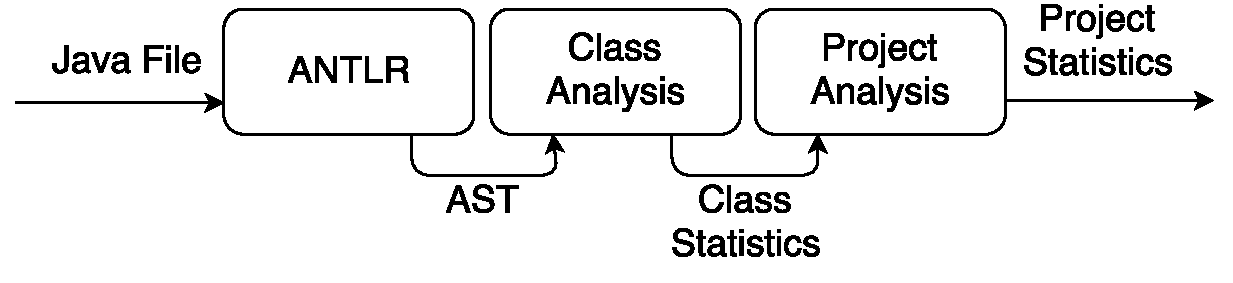
\includegraphics[scale=0.70]{AntlrPipeline.pdf}

The results are then aggregated to produce corpus level analysis which can be found in the following table:
\newline

\captionof{table}{Java Analysis Results}
\begin{tabular}{|l|l|l|l|}
	\hline
	& Count  & \% of classes & \% of extended classes \\ \hline
	Total classes                                                                                   & 116427 &               &                        \\ \hline
	Classes extend another class                                                                    & 71203  & 61.16\%       &                        \\ \hline
	Classes are extended by another class                                                           & 20751  & 17.82\%       &                        \\ \hline
	Classes with forwarding                                                                         & 7087   & 6.09\%        &                        \\ \hline
	\begin{tabular}[c]{@{}l@{}}Classes with forwarding\\ that extend another class\end{tabular}     & 3381   & 2.90\%        &                        \\ \hline
	Classes with downcalls in constructors                                                          & 16101  & 13.83\%       &                        \\ \hline
	Classes storing this in constructors                                                            & 2392   & 2.05\%        &                        \\ \hline
	\begin{tabular}[c]{@{}l@{}}Classes with downcalls or\\ storing this in constructor\end{tabular} & 17099  & 14.69\%       &                        \\ \hline
	\begin{tabular}[c]{@{}l@{}}Extended classes with\\ downcalls in constructors\end{tabular}       & 1545   & 1.33\%        & 7.45\%                 \\ \hline
	\begin{tabular}[c]{@{}l@{}}Extended classes storing\\ this in constructors\end{tabular}         & 178    & 0.15\%        & 0.86\%                 \\ \hline
	Classes with delegation                                                                         & 5183   & 4.45\%        &                        \\ \hline
\end{tabular}

\section{JavaScript}
In JavaScript, there are many ways developers make use of classical inheritance patterns despite the lack of native support in the language. This is largely a result of the numerous libraries which offer their own implementation of classical inheritance behaviour. Some examples of these patterns can be found in the following table:
\captionof{table}{JavaScript Patterns}
\begin{tabular}{|p{5cm}|p{9cm}|}
	\hline
	\multicolumn{2}{|c|}{JavaScript}                                                                                                                                                                  \\ \hline
	Inheritance 1                  & var a = function ( b ) \{    c . call ( this , d );\}                                                                                      \\ \hline
	Inheritance 2                  & function Bar   ( x , y ) \{    Foo . call ( this , x ) ;\}                                                                                 \\ \hline
	Inheritance 3                  & Foo . prototype = object . create ( Bar . prototype )                                                                                      \\ \hline
	Inheritance 4 - Node.js        & var className = defineClass(...)                                                                                                           \\ \hline
	Inheritance 5 - Node.js        & util.inherits(...)                                                                                                                         \\ \hline
\end{tabular}
\newline\newline\newline
The JavaScript analysis in this study makes extensive use of the prior work in developing the JSClassFinder application~\cite{JSClassFinder}. The aim here is to find the cases where JavaScript developers are choosing not to use the native delegation support of the language and are instead modelling their programs with classical inheritance structures. The important factor here is the Class Usage Ratio (CUR) of a JavaScript project as defined in \textit{Does JavaScript Software Embrace Classes?~\cite{JSClassFinder}}. Across a corpus of 50 JavaScript projects, the JSClassFinder returns interesting results about the prevalence of class usage in the language.
\begin{enumerate}
	\item The median CUR across the corpus was 0.15
	\item The upper quartile CUR across the corpus was 0.36
	\item The lower quartile CUR across the corpus was 0.005, which was heavily impacted by 13 systems which had a CUR of zero
\end{enumerate}

\section{Timeline}
The corpora for each of the remaining languages have been collected and the next stage is to analyse each to gather statistics which can be compared to those gathered for Java and JavaScript. The aim is to have a paper ready for the upcoming ECOOP paper submission deadline.
\newline
\captionof{figure}{Project Timeline}
\begin{ganttchart}[
	hgrid,
	vgrid={*{6}{draw=none},dotted},
	x unit=0.87mm,
	group peaks tip position=0,
	group peaks height=.2,
	group peaks width=2,
	time slot format=isodate
	]{2016-07-08}{2016-11-11}
	14
	\gantttitlecalendar{month=shortname} \\
	\ganttgroup{Language Analysis}{2016-07-08}{2016-09-01}\\
		\ganttbar{JavaScript}{2016-07-08}{2016-07-21}\\
		\ganttbar{Python}{2016-07-22}{2016-08-04}\\
		\ganttbar{Scala}{2016-08-05}{2016-08-18}\\
		\ganttbar{Lua}{2016-08-19}{2016-09-01} \\
	\ganttgroup{Collective Analysis}{2016-09-02}{2016-10-13}\\
		\ganttbar{Comparing Analyses}{2016-09-02}{2016-09-23}\\
		\ganttbar{Final Report}{2016-09-02}{2016-10-13}\\
	\ganttgroup{Presentation}{2016-10-14}{2016-11-11}\\
		\ganttbar{Creating Presentation}{2016-10-14}{2016-10-27}\\
		\ganttbar{Rehearsing Presentation}{2016-10-28}{2016-11-11}
\end{ganttchart}
%\chapter{Conclusion}\label{C:con}
The aim of this study was to determine the usefulness of delegation in modern programming languages and whether it could replace classical inheritance. This was achieved by understanding the use of both delegation and classical inheritance to attempt to clarify which model is preferred by developers. This was then followed by an investigation of how difficult it would be to convert projects written in a classical inheritance model over to a delegation model.
\newline

We found that differences between the native support offered by each language and the patterns used by developers of projects in that language were fairly frequent:
\begin{itemize}
	\item In Java, where classical inheritance is natively supported, 6.09\% of classes used forwarding patterns and 4.45\% of classes used delegation patterns. This shows that there is some desire for delegation support from Java developers. Despite this, there remains a much higher use of classical inheritance in these programs which indicates the projects are perhaps better suited to classical inheritance.
	
	\item In C\#, with native support for classical inheritance, analysis showed that the vast majority of classes could be reimplemented in a delegation language with minimal modification. Just 0.17\% of classes contained constructor patterns which would exhibit unexpected behaviour without Uniform Identity. This indicates that replacing a classical inheritance model with delegation could occur with minimal restructuring of existing code.
	
	\item In JavaScript, where delegation is natively supported, 15\% of the functions in the median project were used to emulate class or method behaviour. This use of classes in JavaScript is more than double the use of delegation in Java, implying that developers have a stronger inclination towards class structures than delegation.
	
	\item In Lua, where delegation is natively supported, 17\% of all files contained patterns indicative of class behaviour. This is similar to the statistics for JavaScript, again demonstrating a stronger inclination towards class structures than delegation.
\end{itemize}

From these results, it appears developers have a stronger desire to use classical inheritance structures when provided native delegation than they to use delegation when provided native classical inheritance. It is difficult to determine whether this is because classical inheritance is necessary for aspects of the projects or if its use is simply more common because developers find it more comfortable.
\newline

The further findings of this study involve a measurement of the difficulty involved in reimplementing projects built for classical inheritance into a language built for delegation. The main issues for this reimplementation are constructor patterns which are dependent on Uniform Identity as discussed in Section \ref{inheritanceModels}. It was found, through the Java corpus analysis, that 13.83\% of classes made local calls from constructors and 2.05\% stored \java{this} from a constructor. Through the C\# corpus analysis, it was found that only around 10.3\% of calls to local methods from constructors are dispatched virtually at runtime. In C\#, only 0.17\% of classes contained a call from a constructor to a dynamically dispatched method and 0.94\% of classes store \cs{this} in a constructor. This implies that the total number of cases which would behave differently under delegation would be low, with minimal restructuring required to mitigate this. Thanks to the inclusion of the \cs{virtual} keyword in C\#, its projects would likely be easier to reimplement under delegation.
\newline

The results from the analysis in this study agree with those collected in a range of prior work. The power law distributions of class inheritance usage in Java and C\# line up with the distributions found in \textit{Understanding the Shape of Java Software}. Additionally, the proportion of class usage in Lua as measured by this study compares closely to the JavaScript results found in \textit{Does JavaScript software embrace classes?}. These matching results give weight to our confidence in the correctness of our analysis.

\section{Limitations}
There are some innate limitations to the data which can be gathered through pattern matching against source code as carried out in this study. These limitations are largely a result of two factors. First, the inability to analyse code which is used by, but is not part of, the project; second, the disconnect between how often particular patterns are written (static frequency) and how often they are actually used during execution (dynamic frequency)~\cite{StaticAnalysisLimits}.

\subsection{Inaccessible External Code}
\label{InaccessibleCode}
When only analysing source files, it is difficult to collect information about pre-compiled units which are used by those source files at runtime~\cite{StaticAnalysisLimits}. An example of where this can limit the effectiveness of the analysis in this study is the absence of information about calls dispatched to a superclass when that superclass is defined in a pre-compiled library. If a source code file defines a class \code{A} which extends a class \code{B} where \code{B} is defined in a library with precompiled or otherwise inaccessible source code, we cannot see the details of the methods defined in \code{B}. This becomes an \textsl{}issue because it is no longer possible to determine whether a local call in \code{A} which targets a method defined on \code{B} will be dispatched statically or virtually because we cannot see the method declaration in \code{B}. This could cause unforeseen changes to the behaviour of the methods on \code{A} if another class \code{C} were to extend \code{A} and override methods from \code{B} which we were previously unaware were virtually dispatched calls.

\subsection{Static vs. Dynamic Frequency}
It is difficult, and in some cases impossible, to determine whether any particular class or method is actually used in the execution of a program, or to determine which classes and methods are used more frequently at runtime than others. For example, we might prefer give a different weighting in our analyses to the patterns used in unit test files on the assumption that these are typically written with the expectation that they will rarely need to undergo structural changes after they are written. The are also expected to be executed less frequently than other core functionality in general operation of the program.

\subsection{Incomplete Source Files}
There were cases of files in the JavaScript corpus which could not be parsed in isolation to form a valid syntax tree because they were not syntactically valid source. One example of this was a file which consisted of the majority of a valid JavaScript file but stopped short of the end, with a few other files in the same directory offering several different options for the final part of the code. The assumption here was that the files would be opened and appended at runtime but this was not possible to replicate in a study which operates on source code alone. This study ignored files which could not be compiled on their own, but it is possible that data was lost by ignoring files which expect to be concatenated to create valid programs.

\section{Future Work}
There are a few other methods of software analysis which can work around the issues outlined above to provide a clearer understanding of a software project than analysis based solely on source code.

\subsection{Analysis of Compiled Units}
Analysis of compiled units would help to mitigate the issues explained in section \ref{InaccessibleCode} where precompiled libraries are inaccessable to the analysis. Java and C\# both provide intermediate representations in the form of bytecode languages. For Java this is the Java Bytecode Language~\cite{JVMSpec} and for C\# this is Microsoft's Common Intermediate Language~\cite{CommonIntermediateLanguage}. An analysis of these intermediate representations would be useful because they both offer varied instructions for method calls depending on whether the call is virtually or statically dispatched. This helps to overcome the limitation of being unaware of how a call will be dispatched when analysing source code only.

\subsection{Analysis of Dynamic Frequency}
Analysing a program at runtime could provide useful information about how often particular patterns are used, as opposed to how often they are written. In JavaScript and Lua, a simple way to achieve this would be to modify commonly used libraries associated with classical inheritance implementations to add counters which record how often classes are created, modified or instantiated. In Java, a program called JVM Monitor~\cite{JVMMonitor} could be used to determine the invocation counts of methods which are of interest. This would allow code which is core to the functionality of the program to be weighted more heavily and code which is run relatively infrequently to be weighted more lightly.

\subsection{Measuring Intent}
Ideally, an empirical study of this nature would come with measures of the precision and recall of the algorithm. For this study, these measures would be dependent on comparing the patterns detected by the algorithms against the intent of the developer. Unfortunately, there is no easy way to accurately differentiate between a developer's intent and the patterns they use in their code. This issue is discussed in \textit{Does JavaScript Software Embrace Classes?} where Silva et al. describe the creation of the JSClassFinder tool~\cite{JSClassFinder}. Even when manually inspecting files and analysis results, it is often not possible to determine whether the result of the analysis is truly indicative of the developer's intent. For this reason, it is only possible to approximate the values of precision and recall based on some assumptions about whether certain patterns are, in fact, representative of the behaviours under analysis. Despite this, having estimated ranges of these precision and recall values could help to improve confidence in the research so would be valuable future work.
%\chapter{Some \LaTeX\ hints and tips}\label{C:ex}\LaTeX\ is a very good tool for producing well-structured documents carefully. It is very bad tool for banging things together in a rush and panic. \section{Floats}One perennial problem with \LaTeX\ is its treatment of \emph{floats}.  Suppose you have a figure or table which you want to include in your document. Where should it go? Traditional typesetting practice is to put these in some convenient place, such as the top or bottom of the current or next page, or at the end of the section or chapter.  \LaTeX\ adopts a similar strategy, and allows floats to ``float'' away from where they were defined. You can give a hint about where you want the figure, but \LaTeX\ may move it. Sometimes this is fine but sometimes you may want to have more control and insist that a float goes \emph{here}. Anselm Lingau's \textsf{float} package gives you this flexibility. For example, the following figure is an example of a non-floating float:\begin{fig}[H]
\begin{center}\begin{tabular}{l|lll}$\delta$ & $\mathit{a}$ & $\mathit{b}$ & $\Lambda$ \\ \hline $S_{1}$  & $\{\}$       & $\{\}$      & $\{S_{2}, S_{5}, S_{10}\}$\\$S_{2}$  & $\{S_{3}\}$  & $\{\}$      & $\{\}$\\$S_{3}$  & $\{S_{4}\}$  & $\{\}$      & $\{\}$\\$S_{4}$  & $\{S_{3}\}$  & $\{\}$      & $\{\}$\\$S_{5}$  & $\{\}$       & $\{S_{6}\}$ & $\{\}$\\$S_{6}$  & $\{\}$       & $\{S_{7}\}$ & $\{S_{8}\}$\\$S_{7}$  & $\{S_{6}\}$  & $\{\}$      & $\{\}$\\$S_{8}$  & $\{S_{9}\}$  & $\{\}$      & $\{\}$\\$S_{9}$  & $\{\}$       & $\{S_{8}\}$ & $\{\}$\\$S_{10}$ & $\{S_{11}\}$ & $\{\}$      & $\{\}$\\$S_{11}$ & $\{\}$       & $\{S_{10}\}$& $\{\}$\\ \end{tabular}\caption{The transition function of an NFA with $\Lambda$  transitions}

\end{center}
\end{fig}On the other hand, Figure \ref{Fig:two} is a floating float. 



\begin{fig}[tbh]
\begin{center}\begin{tabular}{l|ll}$\delta''$ & $\mathit{a}$ & $\mathit{b}$ \\ \hline $T_{1}$  & $T_{2}$ & $T_{3}$\\ $T_{2}$  & $T_{4}$ & $T_{5}$\\ $T_{3}$  & $T_{6}$ & $T_{7}$\\ $T_{4}$  & $T_{8}$ & \\$T_{5}$  & $T_{10}$ & \\$T_{6}$  &  & $T_{11}$\\ $T_{7}$  & $T_{3}$ & \\$T_{8}$  & $T_{4}$ & \\$T_{10}$  &  & $T_{5}$\\ $T_{11}$  & $T_{6}$ & \end{tabular}
\caption{The transition function of an FA to accept the same language.}\label{Fig:two}
\end{center}
\end{fig}You can define different types of new floats, and you can have tables of them in the contents pages.\section{URL's}Use \verb=\url= from the \textsf{url} package to typeset URL's. Just using \verb+\texttt+ or \verb+\tt+ does not work:\begin{itemize}\item \verb+\texttt{http://www.mcs.vuw.ac.nz/~neil/}+\item \verb+\url{http://www.mcs.vuw.ac.nz/~neil/}+\end{itemize}Give:\begin{itemize}\item \texttt{http://www.mcs.vuw.ac.nz/~neil/}\item \url{http://www.mcs.vuw.ac.nz/~neil/}\end{itemize}If you use the \textsf{hyperref} package then you can produce PDF files with clickable hyperlinks using \verb=\url=.\section{Graphics and \LaTeX}\LaTeX\ offers rather poor support for the inclusion of graphics. There are lots of ways to include pictorial material in \LaTeX, all of which are deficient in some way or other. Look at \cite{GRM97GC} for a description of them. If your document does need to have pictures in it it is worth thinking about what is needed \emph{before} you generate the pictures.\section{The bibliography}You should build up your bibliography as you go along.  Trying to get the details of the bibliography correct at the end of the project is hard work. Make sure that you record all the relevant details. Beware that material on the internet is likely to change very rapidly. If you are going to include material which is only available on the internet, then you should probably include in the reference the date on which you obtained the document.\section{Run \LaTeX, run}\LaTeX\ builds up information about your document for the table of contents, references and so on at each run. This means that, for example, the table of contents is really the table of contents of the previous compilation. You may need to run \LaTeX\ two or three times to let it catch up with itself. If you have cross references within your bibliography (for example two papers from the same collection, such as \cite{Dum93a,Dum93b}) you may need to run BibTeX more than once. It is also possible that the table of contents file has garbage in it, and will prevent the document from being compiled. This may happen if you have had to abort compilation, due to a bug in the source file. If this is the case then removing the \texttt{.toc} file will usually solve the problem. You will have to fix the original bug, of course.\section{Find out more by\ldots}You can find out more by:\begin{itemize}\item reading any one of a number of books, such as \cite{GMS94,Lam94}. The VUW library has copies of these;\item visiting  the Comprehensive \TeX\ Archive Network (CTAN) at \url{www.ctan.org};\item typing \texttt{latex} into Google.\end{itemize}It is \emph{highly unlikely} that you are the first person who ever wanted to do what you want to do with \LaTeX. Therefore it is likely that someone has already solved your problem: the real key to using  \LaTeX\ well is to make effective use of what other people have done.\section{Summary}In this chapter we explained some things about \LaTeX.

%%%%%%%%%%%%%%%%%%%%%%%%%%%%%%%%%%%%%%%%%%%%%%%%%%%%%%%

\backmatter

%%%%%%%%%%%%%%%%%%%%%%%%%%%%%%%%%%%%%%%%%%%%%%%%%%%%%%%

%\bibliographystyle{ieeetr}
\bibliographystyle{acm}
\bibliography{sample}

\end{document}
